\documentclass[9pt,twoside,lineno]{pnas-new}
% Use the lineno option to display guide line numbers if required.

\templatetype{pnassupportinginfo}

\title{Your main manuscript title}
\author{Author1, Author2 and Author3 (complete author list)}
\correspondingauthor{Corresponding Author name.\\E-mail: author.two@email.com}

% \newcommand\nchainsmin{746}
\newcommand\nchainsmax{2995}
\newcommand\minlargestchainsper{23}
\newcommand\maxlargestchainsper{14}
\newcommand\nspanningchainsmin{}
\newcommand\nspanningchainsmax{}


\begin{document}

%% Comment out or remove this line before generating final copy for submission; this will also remove the warning re: "Consecutive odd pages found".
\instructionspage  

\maketitle

%% Adds the main heading for the SI text. Comment out this line if you do not have any supporting information text.
\SItext


% \subsection*{Subhead}
% Type or paste text here. This should be additional explanatory text such as an extended technical description of results, full details of mathematical models, etc.   
\section{Sensitivity analyses}

In this section, we describe our decision-making process to choose parameters for our phylogenetic analysis and report on the sensitivity of our results to these choices. 

\subsection{Downsampling Swiss sequences}
We aim to include Swiss sequences that are spatio-temporally representative of the Swiss epidemic. Therefore, we down-sample available Swiss sequences proportional to confirmed case counts at the regional (cantonal) level. To assess whether the number of transmission chains saturates as we add more and more sequences, we did a saturation analysis. TODO: add figure and discuss implications.

\subsection{Ratio of foreign to Swiss sequences}
We investigated the sensitivity of transmission chain summary statistics to different ratios of genetically similar context sequences from abroad to focal Swiss sequences. Figure \ref{fig:sensitivity_context_set_size} shows that increasing the ratio of context to focal sequences from 1:1 to 3:1 increases the number of estimated transmission chains and decreases their mean size. However, the greatest differences in estimated transmission chains result from the different assumptions about how to resolve phylogenetic uncertainty (smallest vs. largest plausible chains), not the ratio of foreign to Swiss sequences. Therefore, we chose the 2:1 ratio as a balance of speed (smaller dataset = faster tree search convergence) and information content (larger dataset = more precise estimates of transmission chain import dates). We rely on the difference between the smallest and largest plausible chains picked from one such tree to represent uncertainty in the transmission chains.

\subsection{Transmission chain criteria}
After deciding on a ratio of foreign to Swiss sequences, we investigated the sensitivity of transmission chain summary statistics to our criteria for picking transmission chains. Figure \ref{fig:sensitivity_m_p} shows that increasing the maximum number of exported lineages decreases the number of transmission chains and increases their size. Increasing the maximum consecutive exports has a much smaller effect. But again, these differences are smaller than those resulting from the different assumptions about how to resolve phylogenetic uncertainty (smallest vs. largest plausible chains). Therefore, we chose our criteria to be maximum 3 exported lineages and maximum one consecutive export to allow for some exports but not arbitrarily many. 

% \section*{Heading}
% \subsection*{Subhead}
% Type or paste text here. You may break this section up into subheads as needed (e.g., one section on ``Materials'' and one on ``Methods'').

% \subsection*{Materials}
% Add a materials subsection if you need to.

% \subsection*{Methods}
% Add a methods subsection if you need to.


% %%% Each figure should be on its own page
\begin{figure}
\centering
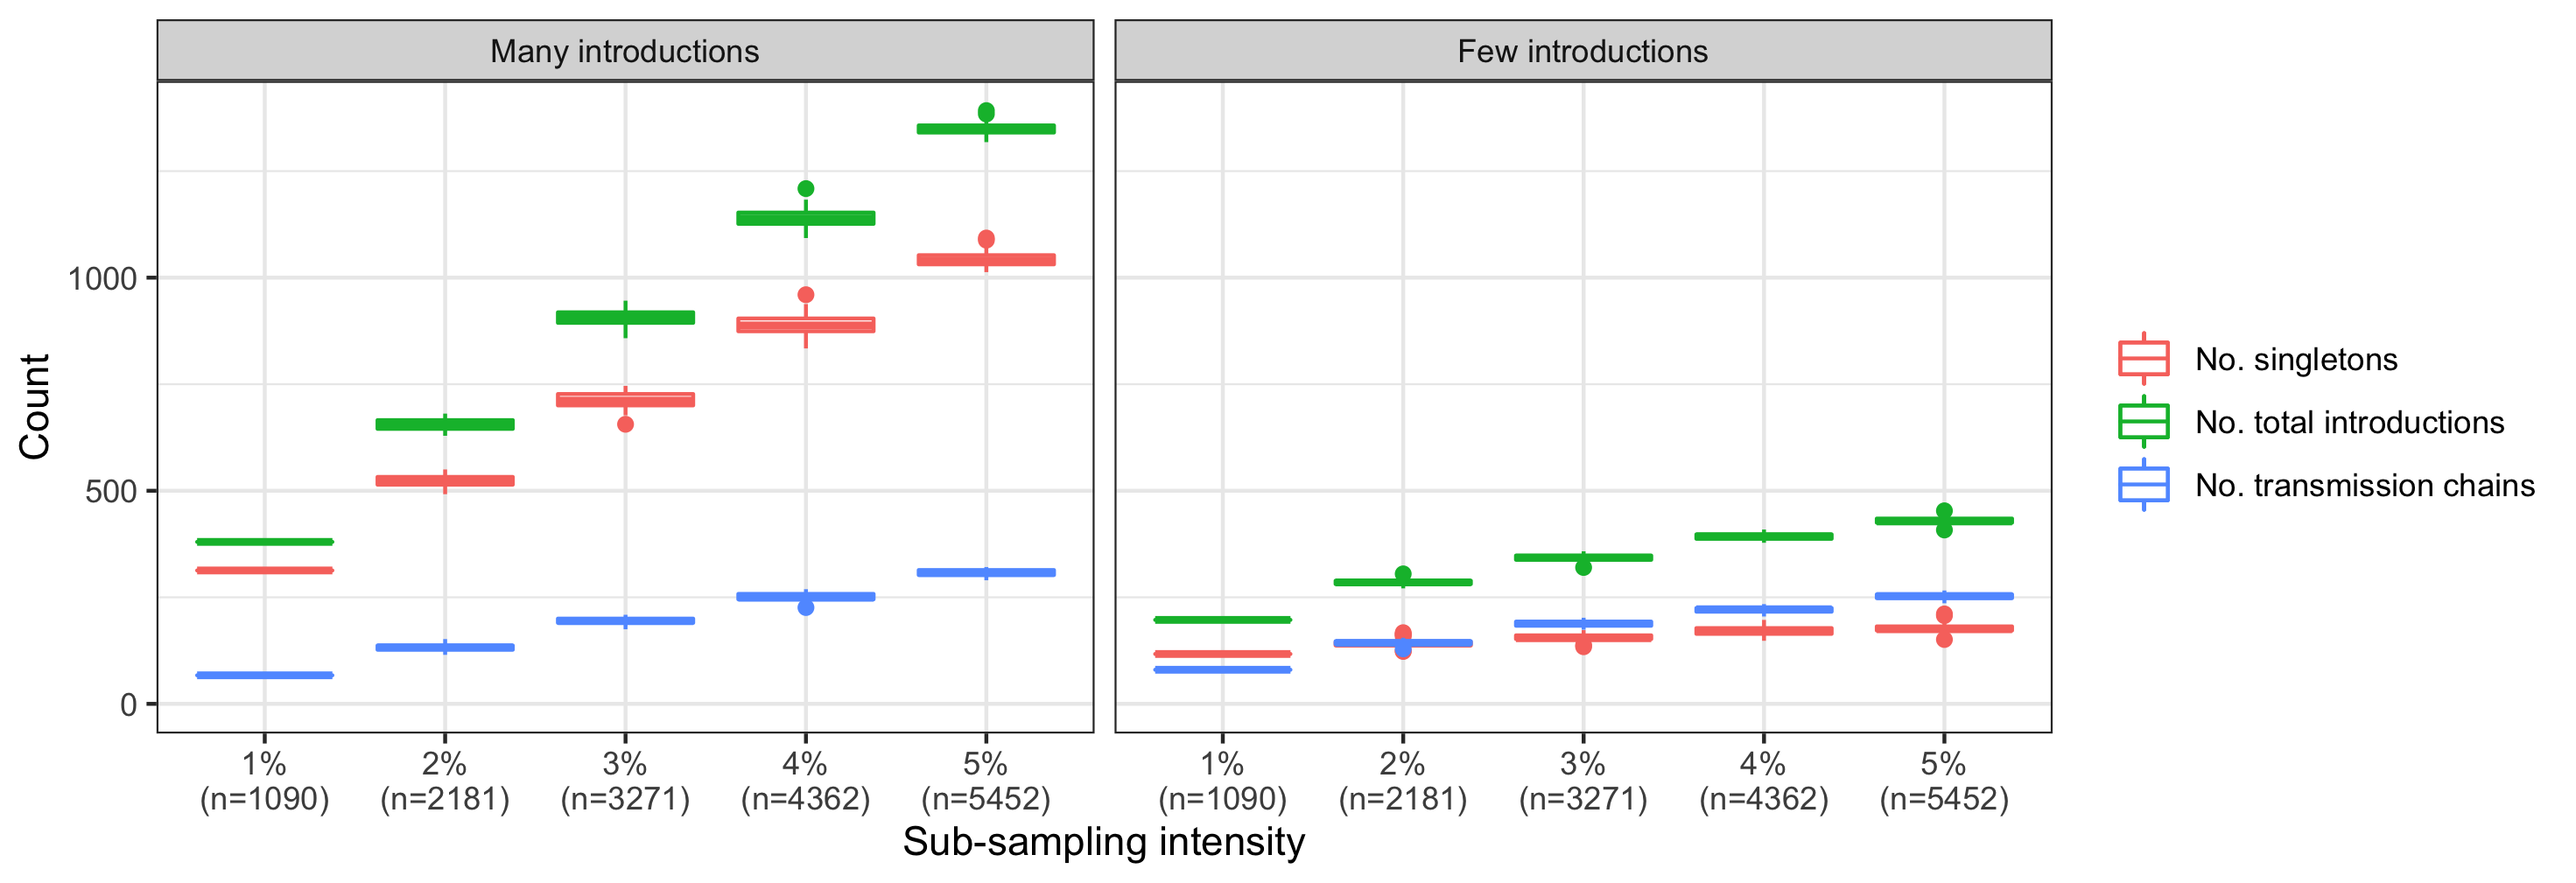
\includegraphics[width = 11.4cm]{figures/fig_SX_sensitivity_subsampling.png}
\caption{Number of estimated introductions as a function of the fraction of Swiss confirmed cases analyzed.}  
\label{fig:sensitivity_downsampling}
\end{figure}

\begin{figure}
\centering
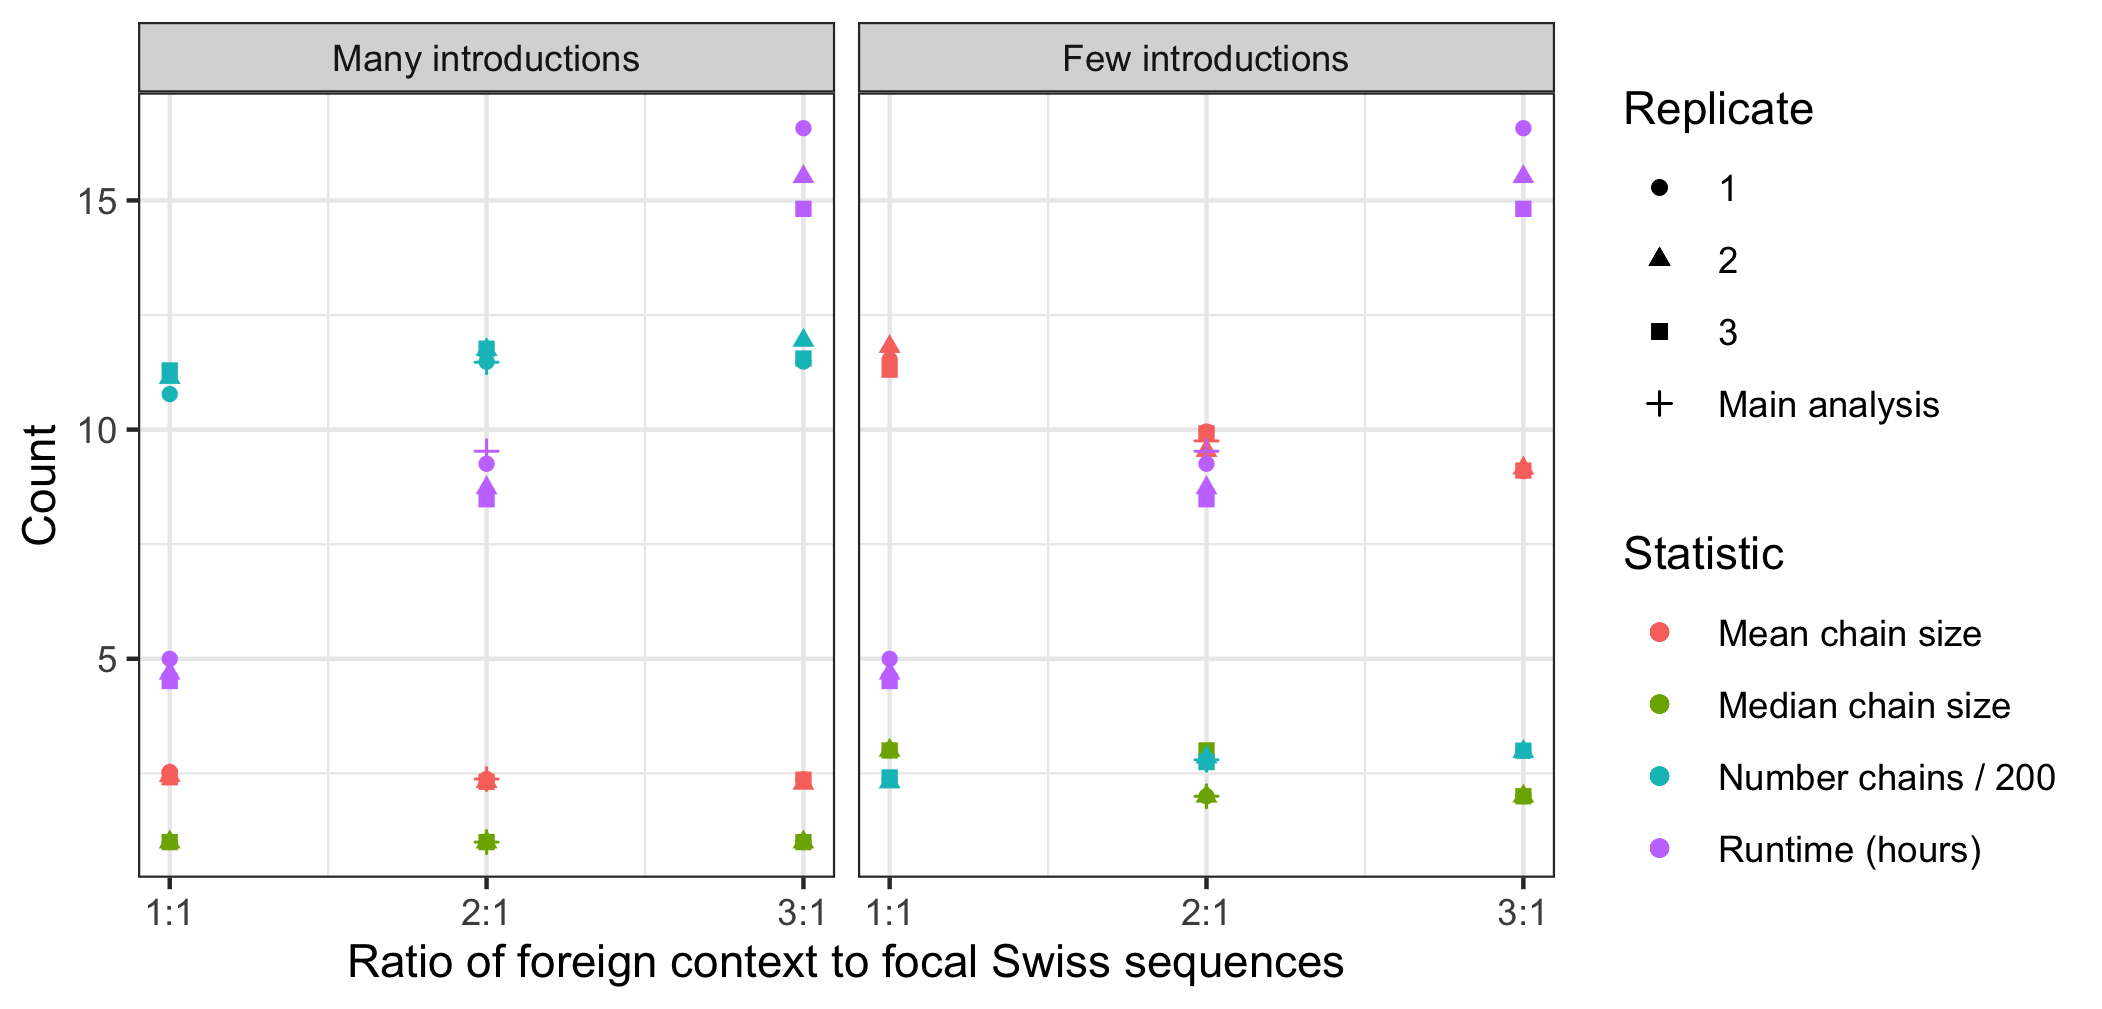
\includegraphics[width = 11.4cm]{figures/fig_SX_sensitivity_context_set_size.png}
\caption{Sensitivity of transmission chain summary statistics to different ratios of focal Swiss sequences to genetically similar foreign context sequences (1:1, 1:2, and 1:3).}  
\label{fig:sensitivity_context_set_size}
\end{figure}

\begin{figure}
\centering
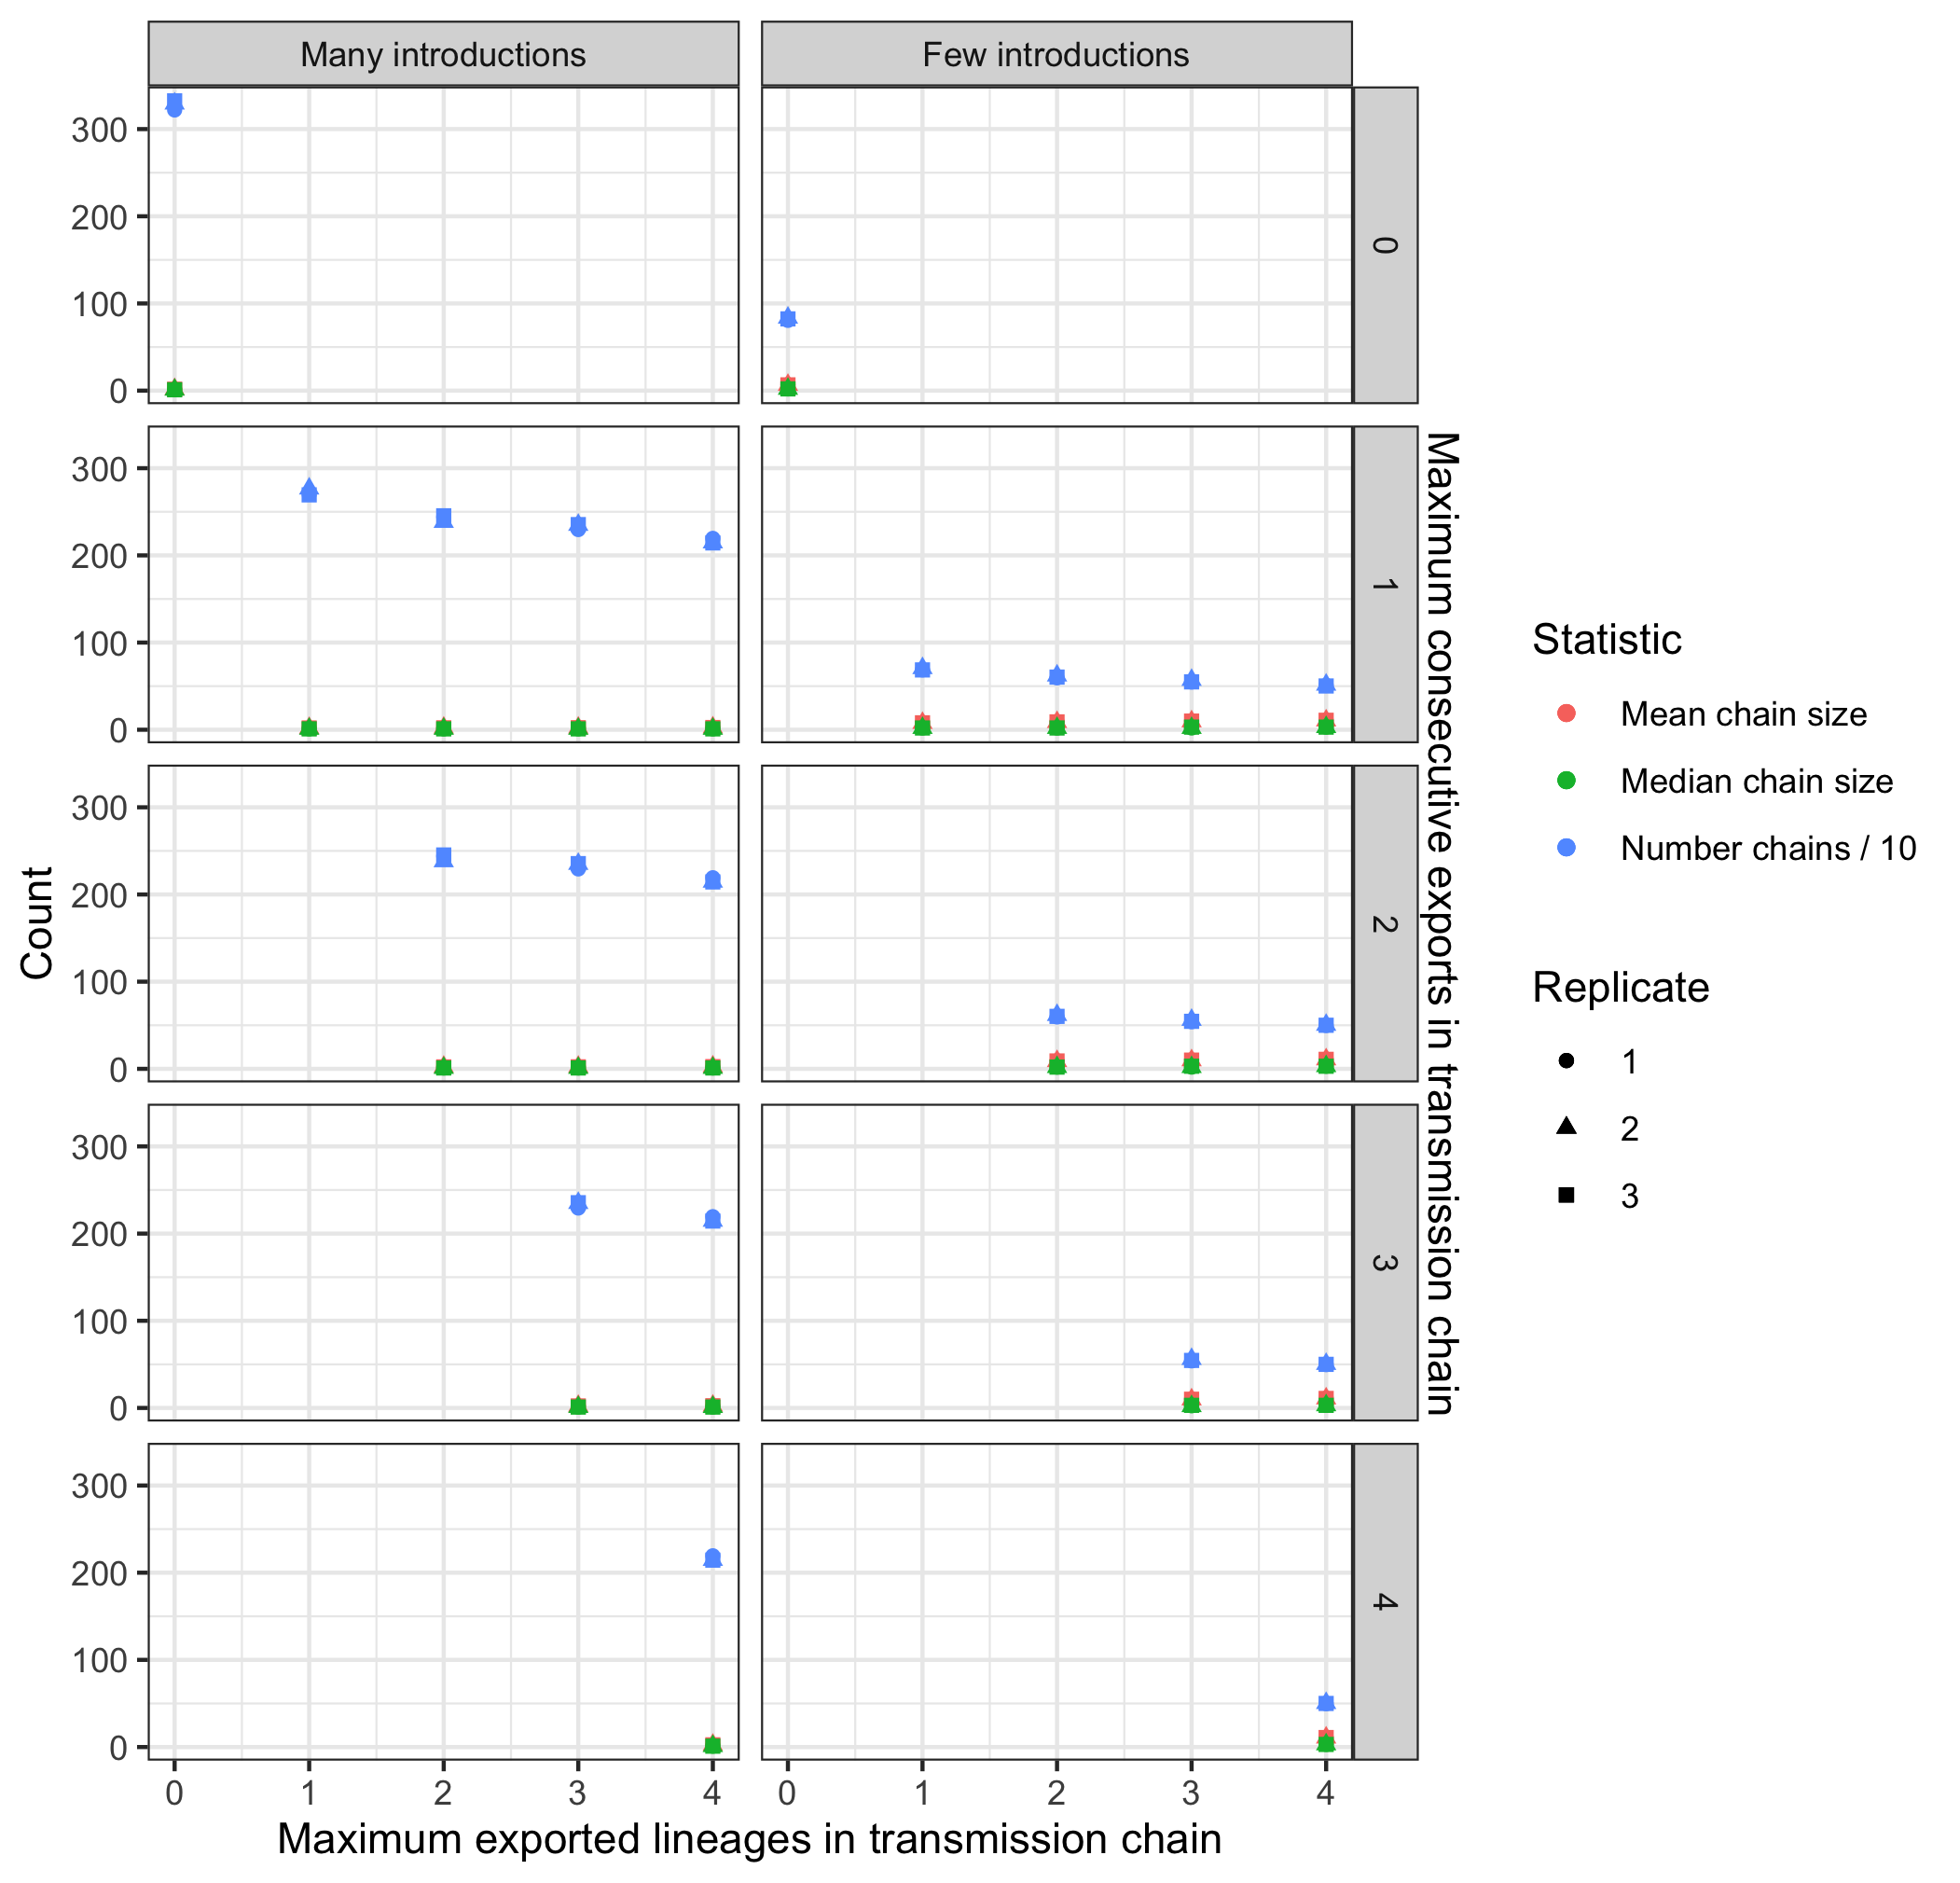
\includegraphics[width = 11.4cm]{figures/fig_SX_sensitivity_chain_defn.png}
\caption{Sensitivity of transmission chain summary statistics to different definitions of a transmission chain.}  
\label{fig:sensitivity_m_p}
\end{figure}

\begin{figure}
\centering
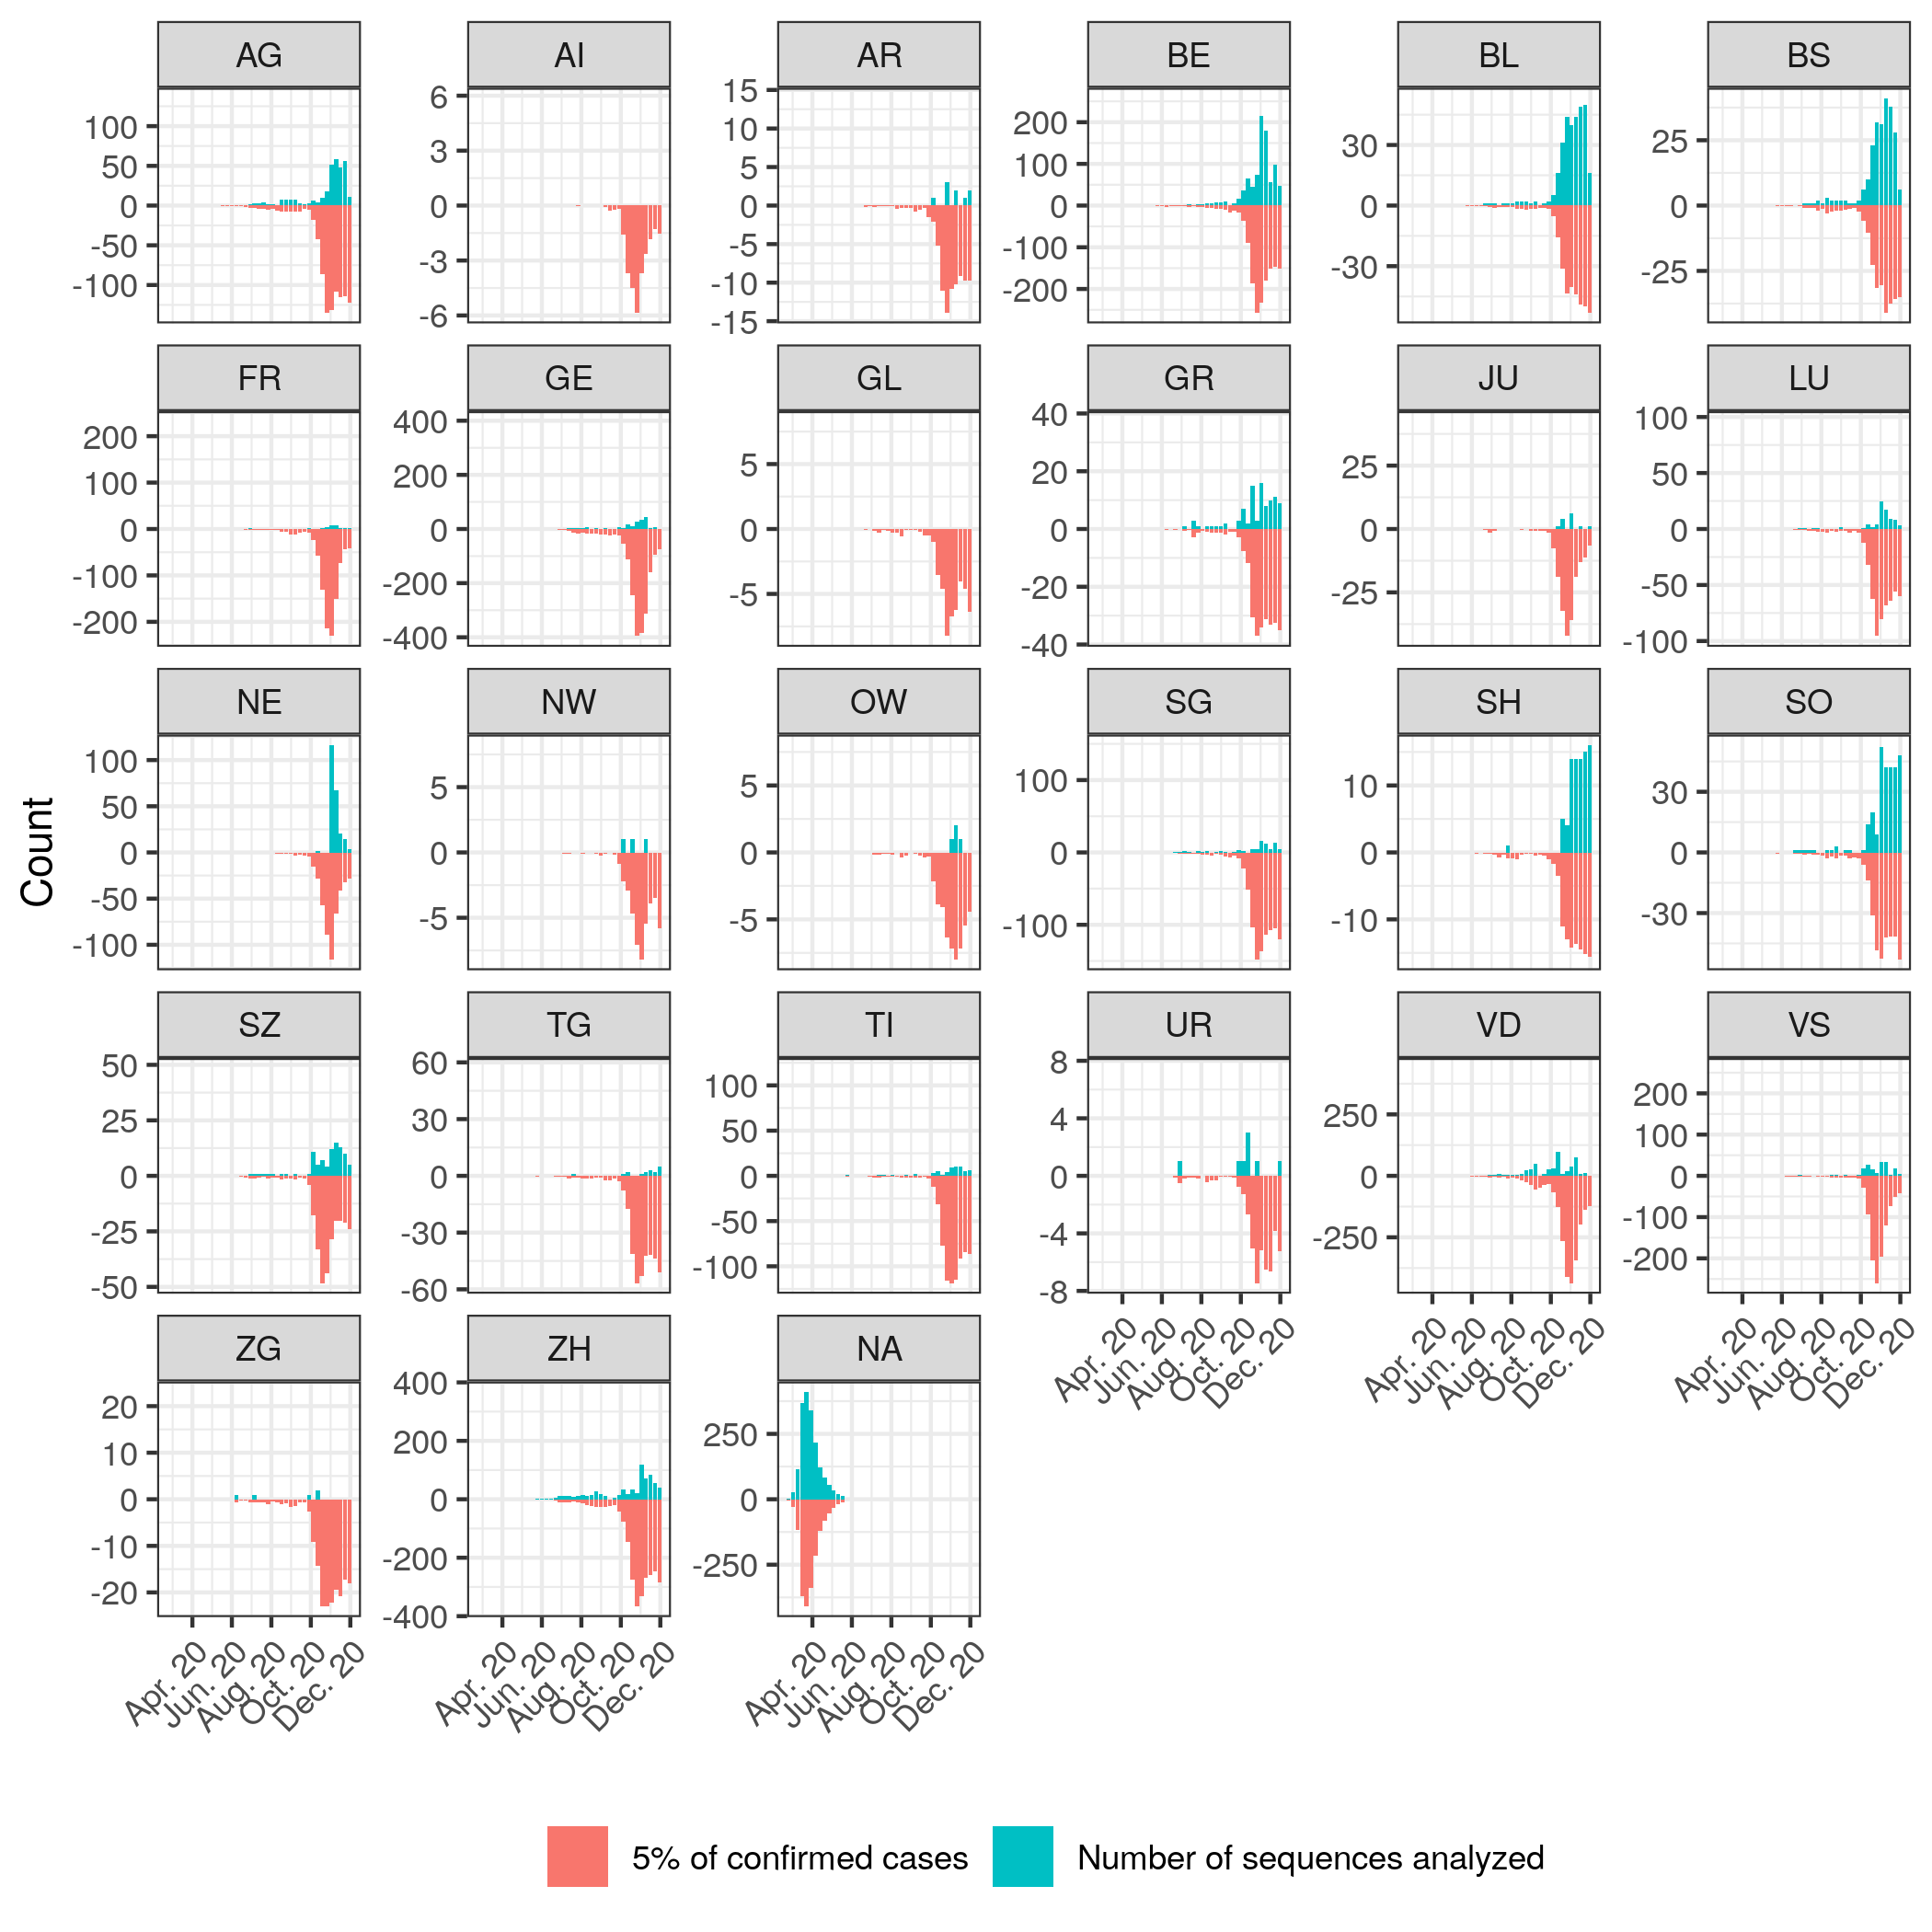
\includegraphics[width = 11.4cm]{figures/swiss_downsampling.png}
\caption{Spatio-temporal representativeness of analyzed genome sequences.}  
\label{fig:downsampling_representativeness}
\end{figure}

% \begin{table}\centering
% \caption{This is a table}

% \begin{tabular}{lrrr}
% Species & CBS & CV & G3 \\
% \midrule
% 1. Acetaldehyde & 0.0 & 0.0 & 0.0 \\
% 2. Vinyl alcohol & 9.1 & 9.6 & 13.5 \\
% 3. Hydroxyethylidene & 50.8 & 51.2 & 54.0\\
% \bottomrule
% \end{tabular}
% \end{table}

% %%% Add this line AFTER all your figures and tables
% \FloatBarrier

% \movie{Type legend for the movie here.}

% \movie{Type legend for the other movie here. Adding longer text to show what happens, to decide on alignment and/or indentations.}

% \movie{A third movie, just for kicks.}

% \dataset{dataset_one.txt}{Type or paste legend here.}

% \dataset{dataset_two.txt}{Type or paste legend here. Adding longer text to show what happens, to decide on alignment and/or indentations for multi-line or paragraph captions.}

% \bibliography{pnas-sample}

\end{document}
